\documentclass[final,hyperref={pdfpagelabels=false}]{beamer}
\usepackage[size=custom,orientation=landscape,width=88,7,height=116,2,scale=1.0]{beamerposter}
\usetheme{I6pd2}
\usepackage[utf8]{inputenc}
\usepackage[frenchb]{babel}
\usepackage{amsmath,amsthm,amssymb,latexsym}
\usepackage{times}\usefonttheme{professionalfonts}
\usefonttheme{serif}
\usepackage{booktabs}
\graphicspath{{figures/}}
\usecaptiontemplate{\small\structure{ }\insertcaption}
\usepackage{multicol}
\usepackage{subfigure}
\setbeamercolor{background canvas}{bg=taaluminium,fg=taaluminium}
%%%%%%% TITLE SECTION %%%%%%%
\title{\huge  Object Removal by Exemplar-Based Inpainting \small Based on Criminisi work}
\author{Di Folco Maxime, GIrot Charly, Jallais Maëliss}
\institute{Ecole Supérieure de Chimie Physique Électronique de Lyon}
%%%%%%%% FOOTER %%%%%%%%
%\newcommand{\foot}{* Criminisi et al : Region filling and object removal by exemplar based image inpainting. IEEE Transactions on image processing, 2004 \hfill \break
%*Bertalmio et al, Image Inpainting. Proceedings of the 27th annual conference on Computer graphics and interactive techniques, 2000. }
%\newcommand{\foot}{\textbf{References} : \hfill \break 



\begin{document}
\addtobeamertemplate{block end}{}{\vspace{2ex}}
\begin{frame}[t]

%%%%%%%% INTRODUCTION %%%%%%%%
\begin{columns}[t]
\begin{column}{.02\textwidth} \end{column}
\begin{column}{.930\textwidth} 
\begin{block}{\Large Introduction}
\begin{columns}[t]
\begin{column}{.496\textwidth}
Objectif
\begin{itemize} 
\item \textbf{Supprimer des objets large} définis par l'utilisateur, à partir d'images numériques. 
\item Corrections d'artefacts ou Restauration d'image
\item Rendu réaliste ou vraisemblable pour l'œil humain
\end{itemize}
Principe
\begin{itemize} 
\item Remplir des régions masquées, par \textbf{propagation de texture} le long des structures linéaires 
\item Utilisation du Principe de \textbf{connectivité} pour définir l'ordre de remplissage : propager les textures tout en conservant les structures linéaires de l'image
\item Recherche de \textbf{patch similaire} par analyse couleur
\end{itemize}

Historique / État de l'art 

 


\end{column}
\begin{column}{.496\textwidth}
\begin{figure}[!b]
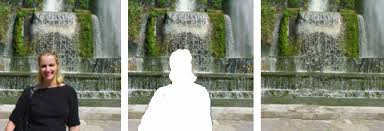
\includegraphics[width=0.8\linewidth]{inpaintingex.jpeg}
\caption{Exemple. De gauche à droite. Originale, Suppression de la région, Remplissage de textures. }
\label{example}
\end{figure}
\end{column}
\end{columns}
\end{block}
\end{column}


\begin{column}{.02\textwidth} \end{column}
\end{columns}

\begin{columns}[t]

\begin{column}{.02\textwidth} \end{column}

\begin{column}{.465\textwidth} 


\begin{block}{\Large Méthodes}
 
\textbf{Algorithme en 3 étapes principales}
\begin{itemize}
%%%%
\item \textbf{Calcul des priorités} en bordure du masque
\begin{itemize}
\item Terme de données * Confiance
\item Terme de données : Quantité de variation des textures autour du pixel courant
\item Confiance : importance accordée au pixel courant
\end{itemize}
%\end{itemize}

\begin{figure}[H]
\centering
\subfigure[Data term itération 0]{\label{fig:data0} 
\includegraphics[width=0.3\textwidth]{figures/0data.png}}
\subfigure[data term itération 4]{\label{fig:data1} 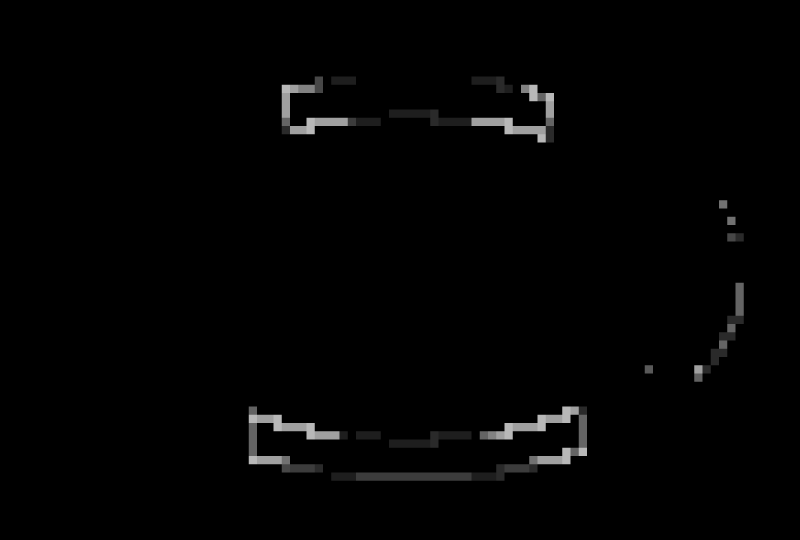
\includegraphics[width=0.3\textwidth]{figures/1data.png}}
\caption{Evolution du terme de données}
\end{figure}

\begin{figure}[H]
\centering
\subfigure[Confiance itération 0]{\label{fig:kabela} 
\includegraphics[width=0.3\textwidth]{figures/0conf.png}}
\subfigure[Confiance itération 4]{\label{fig:kabelb} 
\includegraphics[width=0.3\textwidth]{figures/1conf.png}}
\caption{Evolution de la confiance}
\end{figure}



%%%\\
%\begin{itemize}
\item \textbf{Propagation de la texture et information structurelle}
\begin{itemize}
\item La priorité est donnée aux zones de fortes variations (terme de données)
\item Propager la texture en commencant par ses zones permet de conserver les structures linéaires de l'image
\item les données de textures manquantes autour du pixel de plus forte priorité sont issues de la zone de l'image la plus ressemblante (SSD dans l'espace couleur Lab)
\end{itemize}

\begin{figure}[H]
\centering
\subfigure[image1]{\label{fig:kabela} 
\includegraphics[width=0.3\textwidth]{figures/0oo.png}}
\subfigure[image2]{\label{fig:kabelb} 
\includegraphics[width=0.3\textwidth]{figures/1oo.png}}
\caption{Images à reconstruire sous la forme d'un panorama}
\end{figure}
 
\item \textbf{Mise à jour de la confiance} : les nouveaux pixels copiés obtiennent la confiance du pixel courant de sorte que sa valeur diminue vers l'intérieur du masque indiquant l'incertitude sur la valeur du pixel
\end{itemize}

figures d'actualisation de la confiance 
\end{block}

\end{column}


\begin{column}{.465\textwidth}


\begin{block}{\Large Résultats}

\begin{figure}[H]
\centering
\subfigure[image1]{\label{fig:oval} 
\includegraphics[width=0.4\textwidth]{figures/oval_petit.png}}
\subfigure[image2]{\label{fig:ovalb} 
\includegraphics[width=0.4\textwidth]{figures/resultOvalTest9.png}}
\caption{Inpainting d'une image présentant une occlusion}
\end{figure}

\begin{figure}[H]
\centering
\subfigure[Photo Originale]{\label{fig:lincoln} 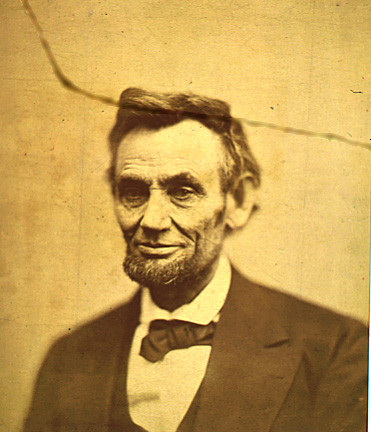
\includegraphics[width=0.4\textwidth]{figures/lincoln.jpg}}
\subfigure[Photo restaurée]{\label{fig:lincolnb} 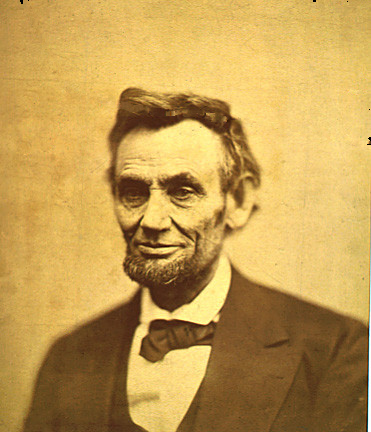
\includegraphics[width=0.4\textwidth]{figures/resultLincoln5bis.png}}
\caption{Restauration d'une image abimée}
\end{figure}
\begin{figure}[H]
\centering
\subfigure[Originale avec occlusion]{\label{fig:troll} 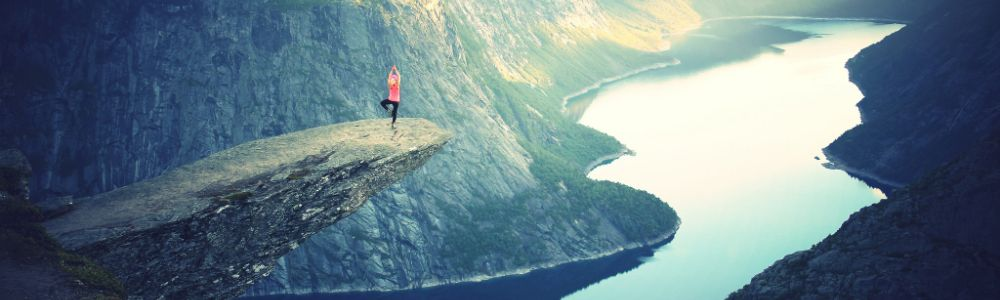
\includegraphics[width=0.4\textwidth]{figures/trolltunga.jpg}}
\subfigure[image2]{\label{fig:trollb} 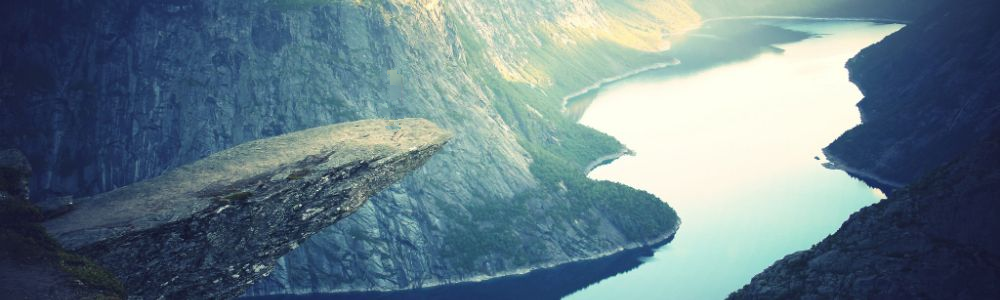
\includegraphics[width=0.4\textwidth]{figures/resultTroll9.png}}
\caption{Suppression d'une personne au milieu d'un paysage}
\end{figure}


\end{block}

\end{column}


\end{columns}

\begin{columns}[t]
\begin{column}{.02\textwidth} \end{column}
\begin{column}{.930\textwidth} 
\begin{block}{\Large Discussion}
\begin{columns}[t]
\begin{column}{.496\textwidth}
\textbf{Limitations}
\begin{itemize}
\item Importance de la \textbf{taille du patch} : Trop grand (pixelise, ne capture pas toutes les variations), trop petit (ne capture pas corréctement les variations des textures plus grande). Doit être légèrement plus grand que le plus grand élément de textures. 
\item Echec de reconstruction sur \textbf{les bordures} de l'image
\item Lab : \textbf{SSD} sous norme CIE 74, échoue parfois à détecter un patch similaire
\end{itemize}


\begin{figure}[H]
\centering
\subfigure[Originale avec occlusion]{\label{fig:order} 
\includegraphics[width=0.3\textwidth]{figures/fillorderd.png}}
\subfigure[Inpainted]{ 
\includegraphics[width=0.3\textwidth]{figures/resultFillOrder35.png}}
\caption{Inpainting de test pour les structures linéaires, démontre l'importance de la taille du patch}
\end{figure}

\end{column}
\begin{column}{.496\textwidth} 
\textbf{Améliorations futures}
\begin{itemize}
\item SSD sous norme CIE 94 ou 2000 - prendre en compte l'uniformité perceptuelle
\item Patch de \textbf{taille variable} pour minimiser la distance à chaue application de texture
\item \textbf{Zone de recherche} du patch à identifier (pas dans toute l'image) - Gain de temps et eventuellement de résultat avec des patchs plus cohérent dans la région proche
\item Interface graphique pour masquage manuel 
\item Utilisation des \textbf{GraphCut} pour séléctionner la meilleure zone à applliquer lors de recouvrement de patch. 
\end{itemize}

\begin{figure}[H]
\centering
\subfigure[Originale]{\label{fig:lake} 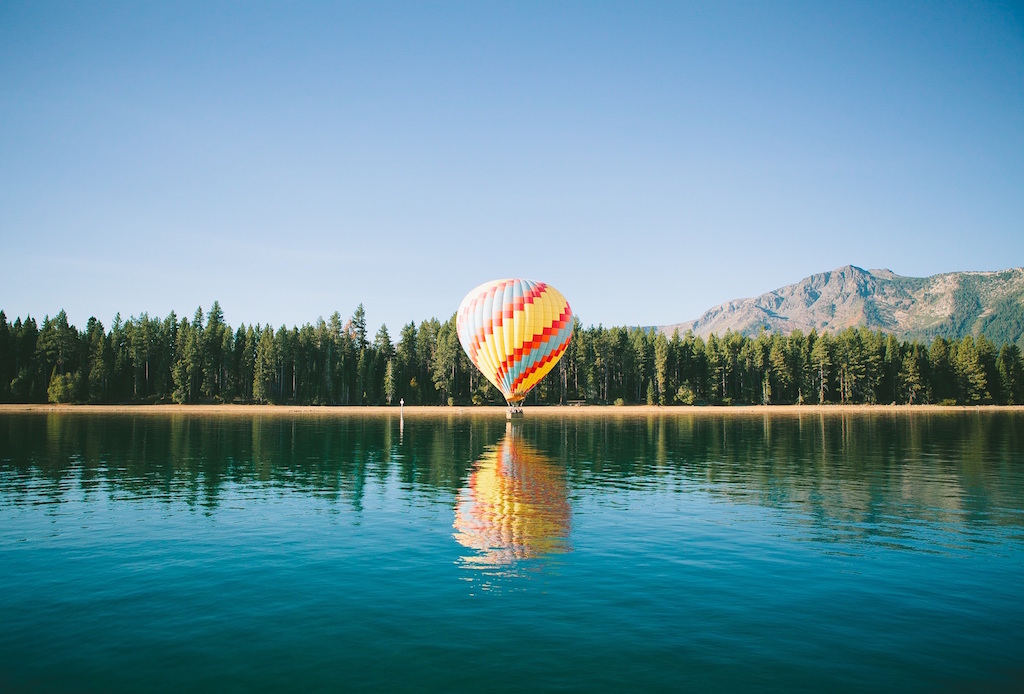
\includegraphics[width=0.24\textwidth]{figures/lakeandballoon.jpg}}
\subfigure[patch taille 5]{\label{fig:lakeb} 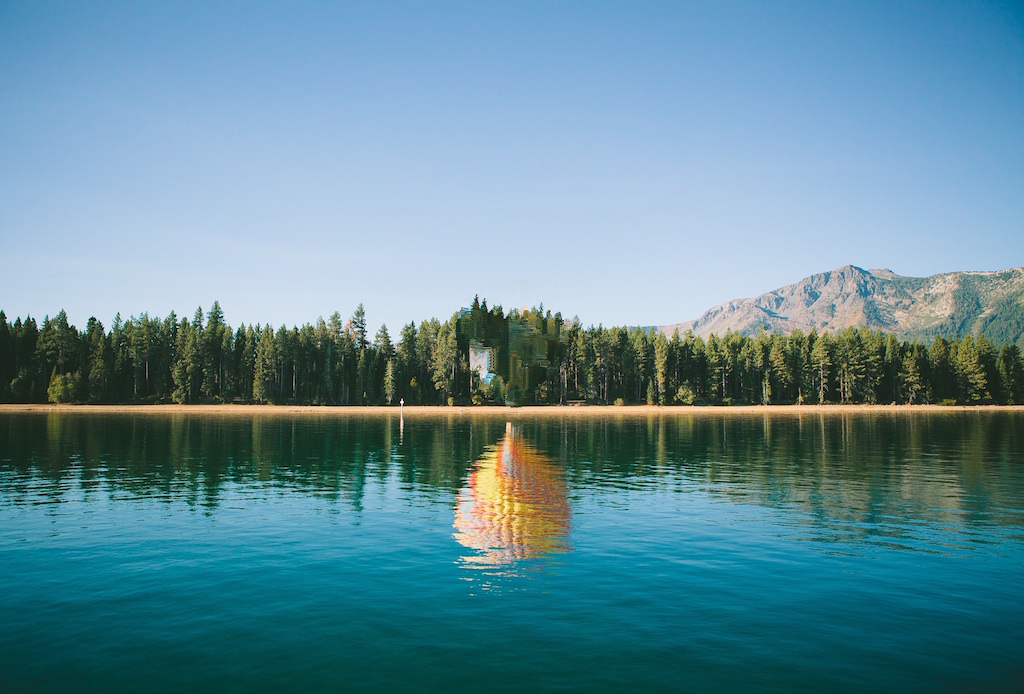
\includegraphics[width=0.24\textwidth]{figures/resultBallon5.png}}
\subfigure[patch taille 13]{\label{fig:lakec}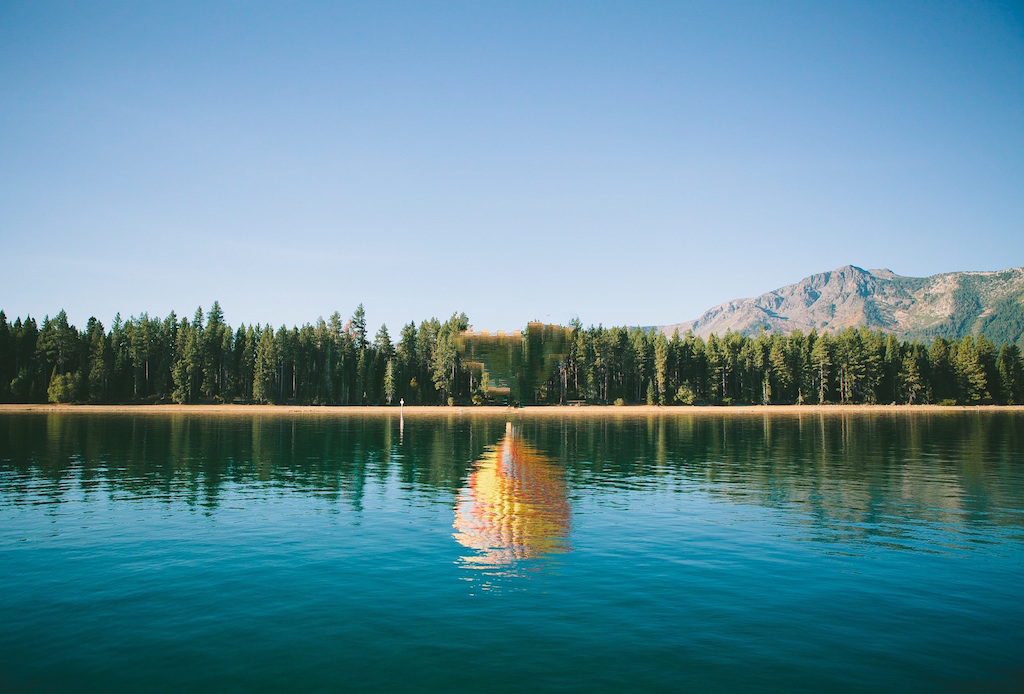
\includegraphics[width=0.24\textwidth]{figures/resultBallon13.png}}
\subfigure[patch 9 et masque complet]{\label{fig:laked}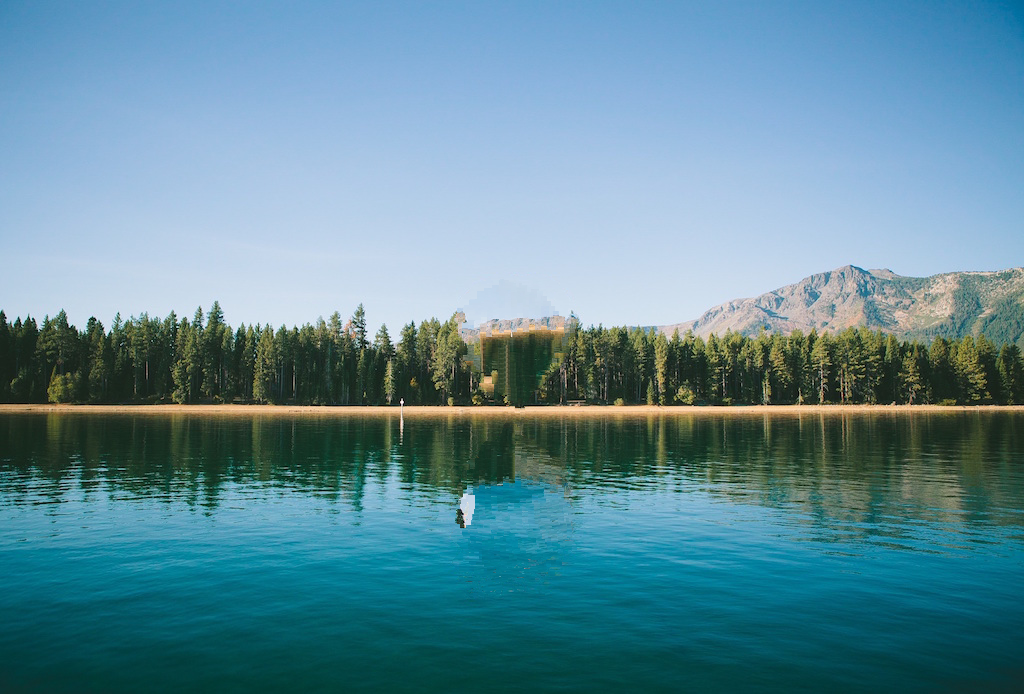
\includegraphics[width=0.24\textwidth]{figures/resultBallonLake9.png}}
\caption{Inpainting d'une montgolfière sur un Lac}
\end{figure}

\begin{block}{Références}
[1] Criminisi et al : Region filling and object removal by exemplar based image inpainting. IEEE Transactions on image processing, 2004 \hfill \break
[2] Bertalmio et al, Image Inpainting. Proceedings of the 27th annual conference on Computer graphics and interactive techniques, 2000.  

\end{block}
\end{column}
\end{columns}
\end{block}
\end{column}
\begin{column}{.02\textwidth} \end{column}
\end{columns}

\end{frame}
\bibliographystyle{\small}
\end{document}
